\iffalse
\let\negmedspace\undefined
\let\negthickspace\undefined
\documentclass[journal,12pt,twocolumn]{IEEEtran}
\usepackage{pgfplots}
\pgfplotsset{compat=1.17}
\usepackage{cite}
\usepackage{amsmath,amssymb,amsfonts,amsthm}
\usepackage{algorithmic}
\usepackage{graphicx}
\usepackage{textcomp}
\usepackage{xcolor}
\usepackage{txfonts}
\usepackage{listings}
\usepackage{enumitem}
\usepackage{mathtools}
\usepackage{gensymb}
\usepackage{comment}
\usepackage[breaklinks=true]{hyperref}
\usepackage{tkz-euclide} 
\usepackage{listings}
\usepackage{gvv}                                        
\def\inputGnumericTable{}                                 
\usepackage[latin1]{inputenc}                                
\usepackage{color}                                            
\usepackage{array}                                            
\usepackage{longtable}                                       
\usepackage{calc}                                             
\usepackage{multirow}                                         
\usepackage{hhline}                                           
\usepackage{ifthen}                                           
\usepackage{lscape}
\newtheorem{theorem}{Theorem}[section]
\newtheorem{problem}{Problem}
\newtheorem{proposition}{Proposition}[section]
\newtheorem{lemma}{Lemma}[section]
\newtheorem{corollary}[theorem]{Corollary}
\newtheorem{example}{Example}[section]
\newtheorem{definition}[problem]{Definition}
\newcommand{\BEQA}{\begin{eqnarray}}
\newcommand{\EEQA}{\end{eqnarray}}
\newcommand{\define}{\stackrel{\triangle}{=}}
\theoremstyle{remark}
\newtheorem{rem}{Remark}
\begin{document}
\bibliographystyle{IEEEtran}
\vspace{3cm}
\title{GATE GE 81Q}
\author{EE23BTECH11021 - GANNE GOPI CHANDU$^{*}$% <-this % stops a space
}
\maketitle
\bigskip
\renewcommand{\thefigure}{\theenumi}
\renewcommand{\thetable}{\theenumi}
\bibliographystyle{IEEEtran}
\textbf{Question}\\
The value of the convolution of $f(x) = 3\cos(2x)$ and $g(x) = \frac{1}{3}\sin(2x)$ where $x \in [0, 2\pi)$, at $x = \frac{\pi}{3}$, is (Rounded off to 2 decimal places)\\
\textbf{Solution}\\
\fi
\begin{align}
    f\brak{w}&=3\cos\brak{2w}\\
    &=\frac{3}{2}e^{j2w}+\frac{3}{2}e^{-j2w} \label{eqge.81.2}\\
    f\brak{w}&=\sum_{k=-\infty}^{\infty}c_k e^{-j w k} \label{eqge.81.3}
\end{align}
   \text{by comparing} \eqref{eqge.81.2} and \eqref{eqge.81.3} \\
\begin{align}
   c_2&=c_{-2}=\frac{3}{2}\\
   c_{k}&=0 \quad{o.w}
\end{align}
\begin{align}
    g\brak{w}&=\frac{1}{3}\sin\brak{2w}\\
    &=\frac{1}{6j}e^{j2w}-\frac{1}{6j}e^{-j2w} \label{eqge.81.7} \\
    g\brak{w}&=\sum_{k=-\infty}^{\infty}d_{k} e^{-j w k} \label{eqge.81.8}
\end{align}
   \text{by comparing} \eqref{eqge.81.7} and \eqref{eqge.81.8} \\
\begin{align}
   d_{2}&=\frac{-1}{6j}\\
   d_{-2}&=\frac{1}{6j}\\
   d_{k}&=0 \quad{o.w}
\end{align}
The periodic convolution is multiply Fourier series coefficients is
c\brak{n}=c\brak{k}*d\brak{k}*p\\
\begin{align}
    c_{2}&=c_{2}*d_{2}*p\\
    &=\brak{\frac{3}{2}}\brak{\frac{-1}{6j}}\brak{2\pi}\\
    &=\frac{-\pi}{2j}
\end{align}
and
\begin{align}
    c_{-2}&=c_{-2}*d_{-2}*p\\
    &=\brak{\frac{3}{2}}\brak{\frac{1}{6j}}\brak{2\pi}\\
    &=\frac{\pi}{2j}
\end{align}
\begin{align}
   {f*g}\brak{x}&=\sum_{n=-N}^{N}c_{n} e^{-j\frac{2\pi nx}{p}}\\
    &=c_{-2}e^{j2x} + c_{2}e^{-j2x}\\
    &=\frac{\pi}{2j}e^{j2x}-\frac{\pi}{2j}e^{-j2x}\\
    &=\frac{\pi}{2j}\brak{e^{j2x}-e^{-j2x}}\\
    &=\frac{\pi}{2j}\brak{sin\brak{2x}2j}\\
    &=\pi \sin\brak{2x}\\
\end{align}
at $x=\frac{\pi}{3}$
\begin{align}
    &=\frac{\sqrt{3}\pi}{2}\\
    &\approx 3
\end{align}
Therefore the convolution of f(x) and g(x) is 3
\begin{figure}[!h]
    \centering
    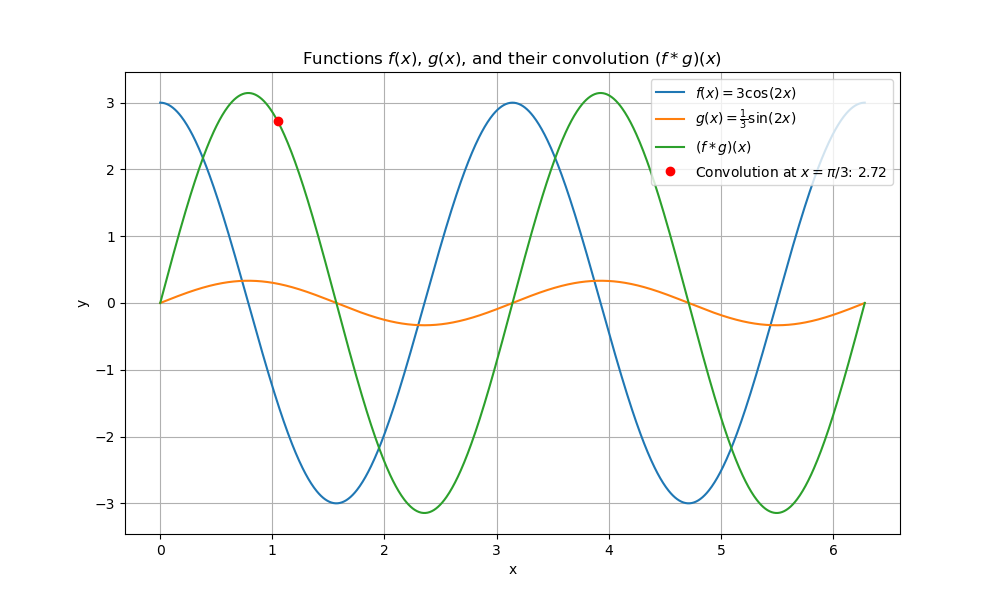
\includegraphics[width=1.0\linewidth]{2023/GE/81/figs/ga.81.png}
    \caption{Plot of y vs x}
    \label{fig:1}
\end{figure}
